\chapter{PERANCANGAN SISTEM}
\label{bab:perancangan-sistem}

Bab ini menjelaskan pelaksanaan penelitian berdasarkan data, implementasi, dan konfigurasi eksperimen yang tersedia. Sistem yang dirancang merupakan alur eksperimen deteksi objek. Masukannya adalah citra jalan dan anotasi, sedangkan keluarannya berupa model terlatih, prediksi, serta metrik evaluasi.

\section{Desain Perancangan Sistem}
Penelitian menggunakan desain komparatif dengan tiga fokus yang mengikuti rumusan masalah. Fokus pertama adalah kinerja deteksi pada domain sumber beserta perbandingan penggunaan kelas pengecoh. Fokus kedua adalah keseimbangan ketepatan dan kebutuhan komputasi. Fokus ketiga adalah kemampuan generalisasi pada citra jalan Indonesia tanpa pelatihan ulang.

Lima model dibandingkan pada pembagian data sumber yang sama. Data latih digunakan untuk pembaruan parameter dan perhitungan bobot kelas. Data validasi digunakan untuk pemantauan, penghentian dini, dan pemilihan \textit{checkpoint}. Data uji sumber digunakan untuk pelaporan kinerja akhir. Data target digunakan hanya untuk pengujian lintas domain, tanpa pembaruan bobot model.

Rancangan mempertahankan tujuan proposal, dengan beberapa penyesuaian sesuai pelaksanaan. Model modifikasi direalisasikan sebagai rekonstruksi YOLOv8-PD dan YOLO-RD. Penanganan ketimpangan menggunakan pembobotan jumlah efektif sampel. Pengujian target mencakup seluruh model, sehingga peringkat sumber dan target dapat diperiksa bersama. Jumlah data target yang dievaluasi adalah 307 citra, berbeda dari target pengumpulan minimal 500 citra pada proposal.

\section{Diagram Blok}
Alur pemrosesan sumber dan target ditunjukkan pada Gambar~\ref{fig:alur-penelitian}. Jalur target menggunakan model yang telah dipilih melalui validasi sumber.
\begin{figure}[H]
\centering
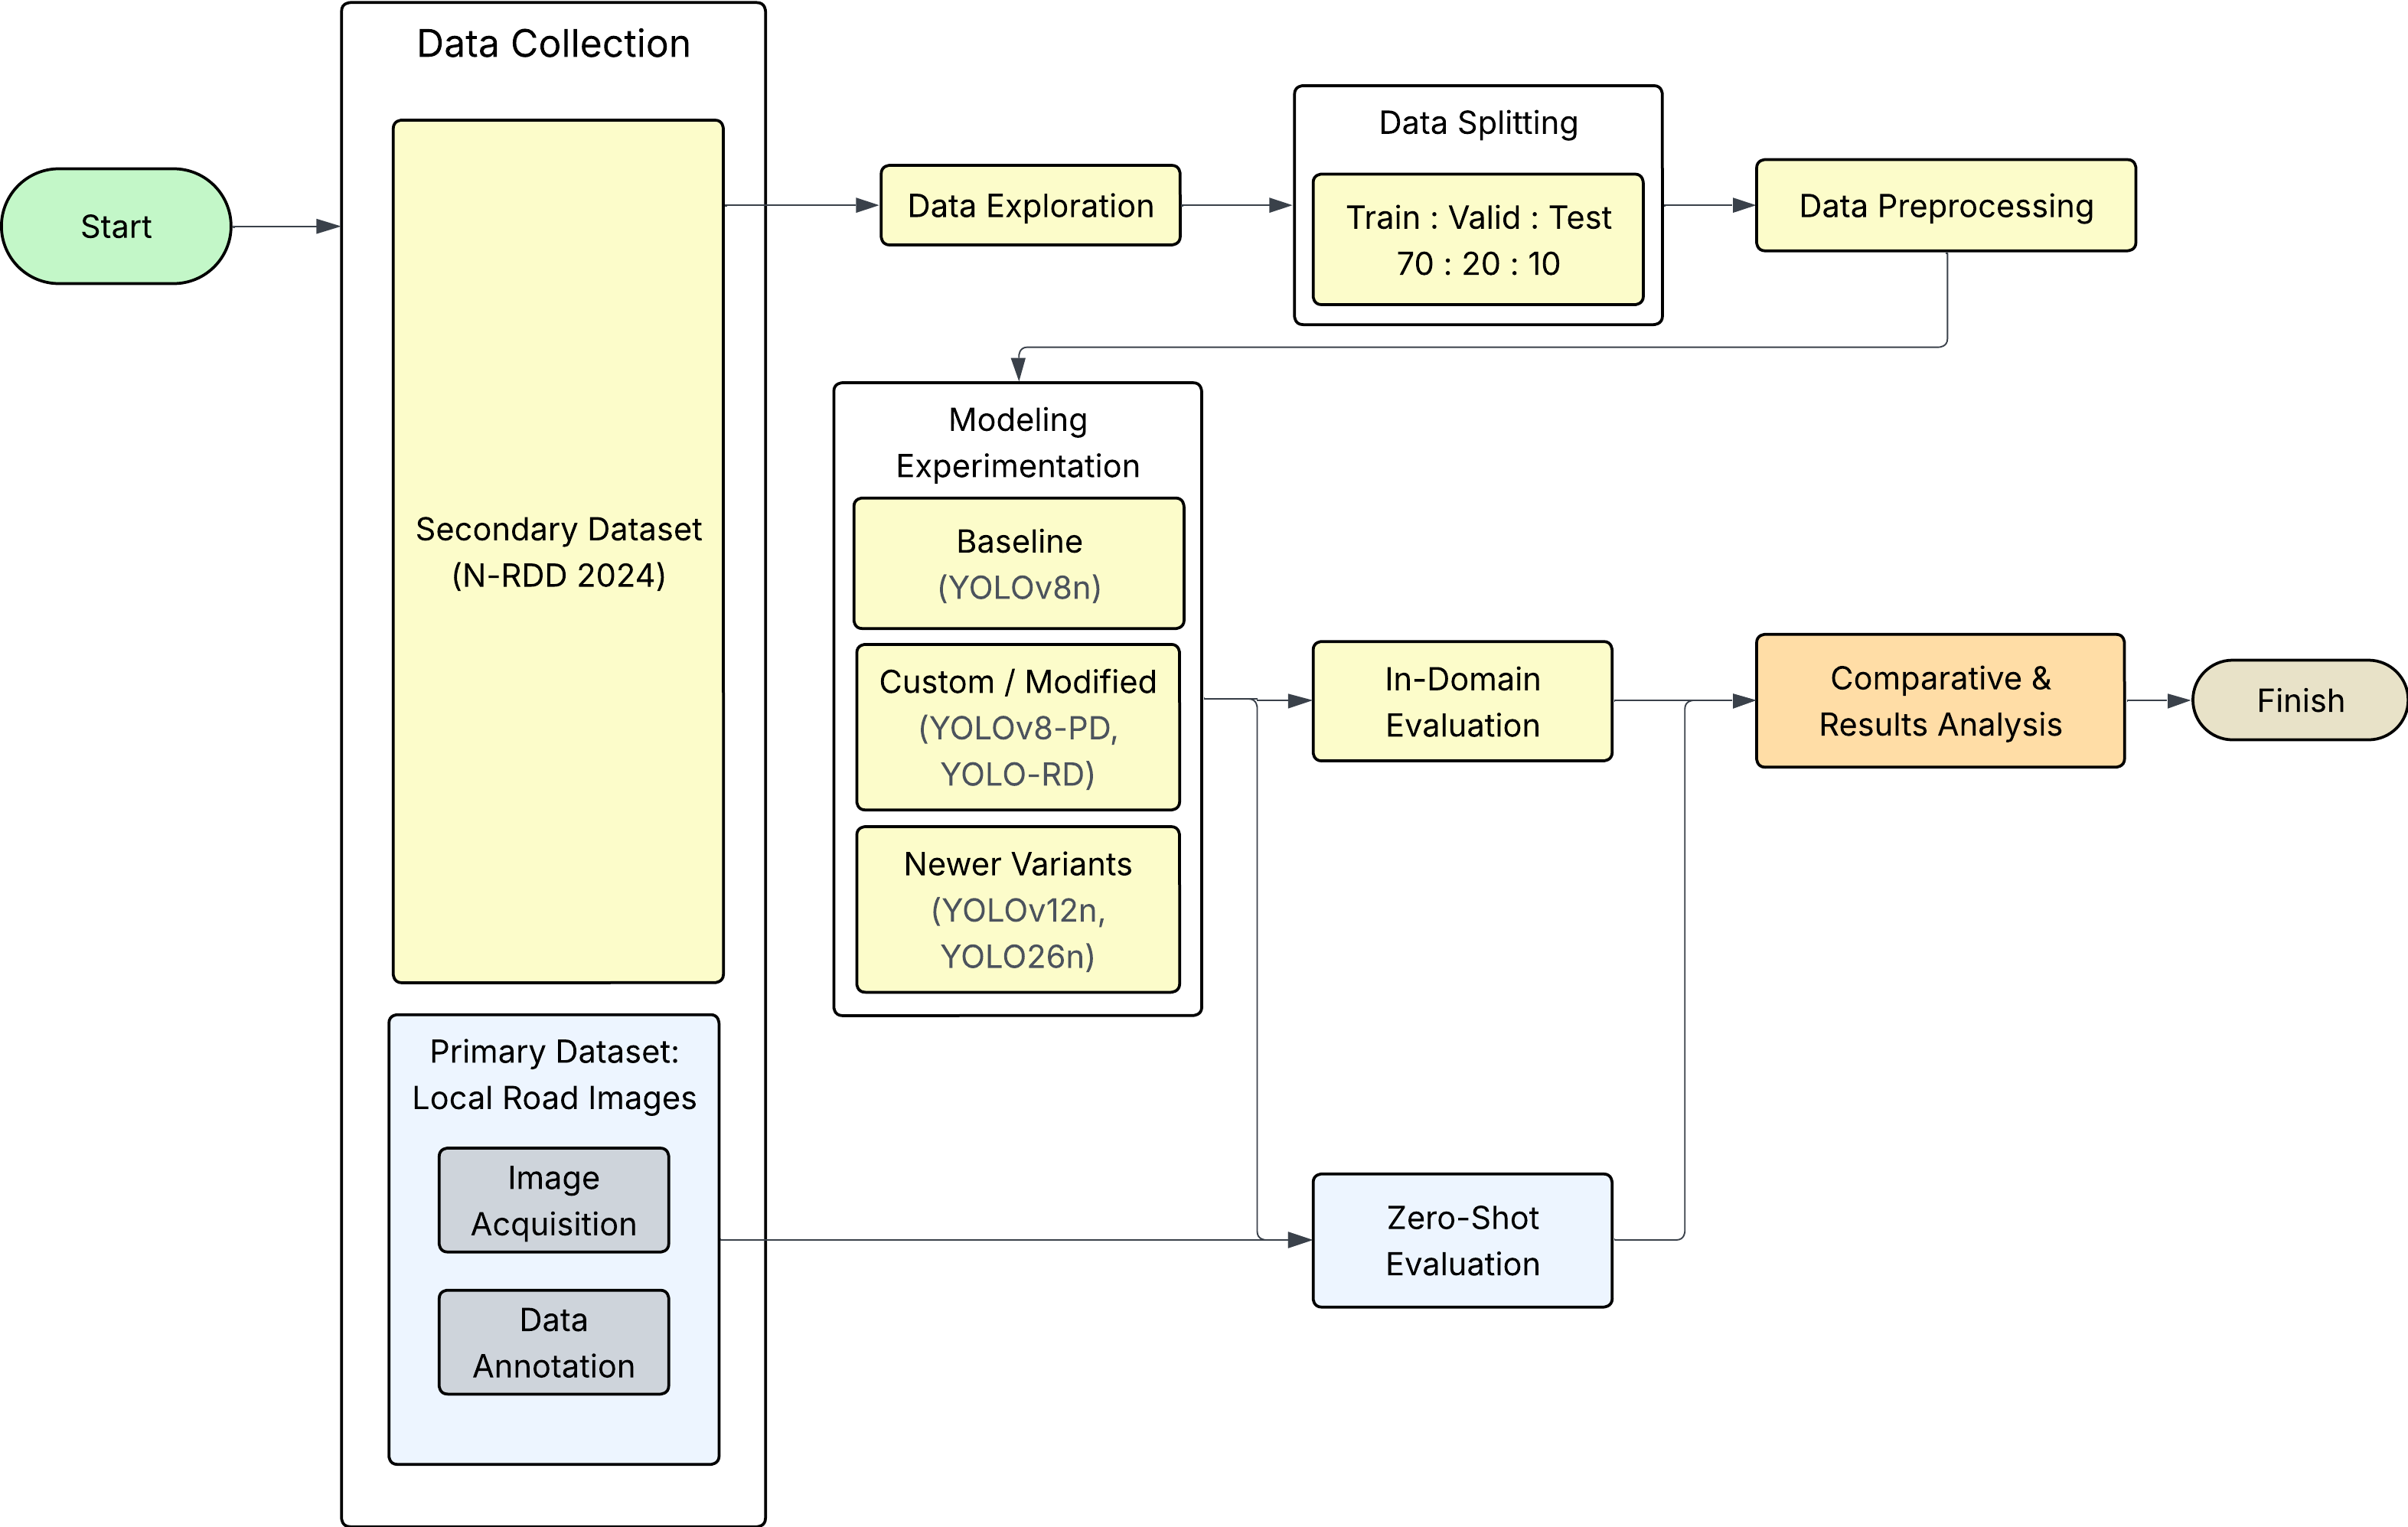
\includegraphics[width=\linewidth]{methodology_workflow.png}
\caption{Alur eksperimen komparatif dan pengujian lintas domain.}
\label{fig:alur-penelitian}
\end{figure}
Gambar~\ref{fig:alur-penelitian} membedakan jalur data sekunder untuk pelatihan dari data primer untuk evaluasi \textit{zero-shot}. Pada jalur data primer, akuisisi diikuti anotasi sebelum evaluasi. Jalur pemodelan memasok bobot terbaik berdasarkan validasi sumber, tanpa pembaruan bobot pada target. Kelompok \textit{custom/modified} pada diagram merujuk pada rekonstruksi YOLOv8-PD dan YOLO-RD. Rasio 70:20:10 merupakan proporsi rencana; jumlah aktual dijelaskan pada bagian pembagian data.

Evaluasi sumber mencakup ketepatan deteksi dan efisiensi komputasi. Eksperimen empat kelas menjadi analisis tambahan pada domain sumber, sedangkan pengujian target menggunakan bobot pelatihan utama enam kelas. Perbandingan lintas domain dirangkum pada empat kelas kerusakan yang sama.

\section{Fungsi dan Fitur}
Alur eksperimen menyediakan fungsi penyiapan data, pelatihan, evaluasi, dan pemeriksaan prediksi. Penyiapan data mencakup penyaringan kelas serta penyelarasan identitas kategori. Pelatihan menghasilkan bobot setiap model dengan pencatatan argumen dan perkembangan metrik. Evaluasi menghasilkan metrik agregat, metrik per kelas, serta ringkasan waktu pemrosesan.

Pemeriksaan prediksi digunakan untuk membaca contoh deteksi benar, objek terlewat, dan prediksi yang tidak sesuai anotasi. Analisis tambahan membandingkan pelatihan empat dan enam kelas serta menghitung prediksi lubang yang bertumpang tindih dengan anotasi pengecoh. Keluaran tersebut mendukung interpretasi hasil, tetapi contoh visual tidak diperlakukan sebagai ukuran frekuensi kesalahan seluruh dataset.

\section{Desain Perangkat Keras dan Lunak}
Implementasi menggunakan Python, PyTorch, dan kerangka Ultralytics. Model rekonstruksi menggunakan modul tambahan yang didaftarkan pada pemuat arsitektur Ultralytics. Anotasi target dikelola menggunakan Roboflow. Lingkungan pengukuran kecepatan sumber dirangkum pada Tabel~\ref{tab:lingkungan}.
\begin{table}[H]
\centering
\caption{Lingkungan evaluasi untuk pengukuran kecepatan sumber.}
\label{tab:lingkungan}
\begin{tabularx}{\linewidth}{|l|X|}\hline
\rowcolor{black}\HeaderTabel{Komponen}&\HeaderTabel{Konfigurasi tercatat}\\\hline
GPU & NVIDIA GeForce RTX 4070 SUPER, memori 12 GB\\\hline
Python & 3.12.3\\\hline
PyTorch dan CUDA & PyTorch 2.5.1; CUDA 12.1\\\hline
Ultralytics & 8.4.108\\\hline
Ukuran masukan & 640 piksel\\\hline
Data pengukuran & Data uji sumber, 995 citra\\\hline
\end{tabularx}
\end{table}
Tabel~\ref{tab:lingkungan} mengikuti log evaluasi sumber yang menjadi dasar estimasi FPS. Konfigurasi tersebut tidak digeneralisasi sebagai lingkungan seluruh eksperimen tambahan. Penghitungan ulang kompleksitas model menggunakan Ultralytics 8.4.177 dan dipisahkan dari pengukuran waktu yang tercatat pada versi 8.4.108.

\section{Data dan Prapemrosesan}
\subsection{Akuisisi dan seleksi data sumber}
Data sekunder berasal dari N-RDD2024~\cite{kaya2024nrdd2024}. Sesuai eksplorasi pada proposal, subset Asia awal berjumlah 10.395 citra. Penyaringan mempertahankan citra yang memiliki sedikitnya satu objek dari enam kelas penelitian dan menghasilkan 9.670 citra. Anotasi di luar kategori tersebut tidak digunakan dalam pelatihan.

Distribusi citra sumber terdiri atas 6.638 citra Jepang, 1.977 citra Tiongkok, dan 1.055 citra India. Proporsinya ditunjukkan pada Gambar~\ref{fig:distribusi-negara}.
\begin{figure}[H]
\centering
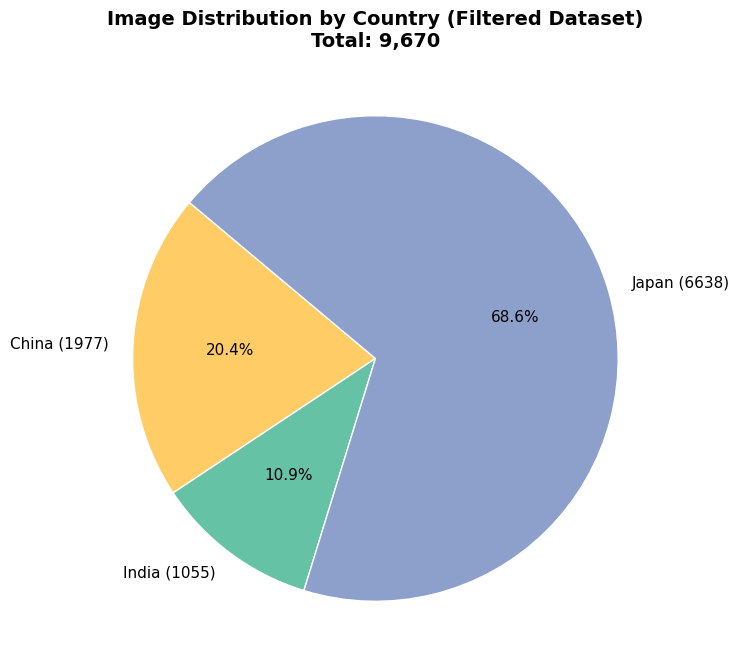
\includegraphics[width=.76\linewidth]{distribusi_gambar.png}
\caption{Distribusi citra sumber menurut negara, digunakan kembali dari eksplorasi data proposal.}
\label{fig:distribusi-negara}
\end{figure}
Gambar~\ref{fig:distribusi-negara} memperlihatkan bahwa kontribusi jumlah citra ketiga negara tidak sama. Komposisi ini perlu dipertimbangkan saat membaca hasil agregat. Proporsi citra bukan ukuran kesamaan karakteristik jalan suatu negara dengan Indonesia.

Contoh anotasi enam kelas disajikan pada Gambar~\ref{fig:contoh-kelas}. Setiap panel memperlihatkan contoh kategori, bukan hasil prediksi model.
\begin{figure}[H]
\centering
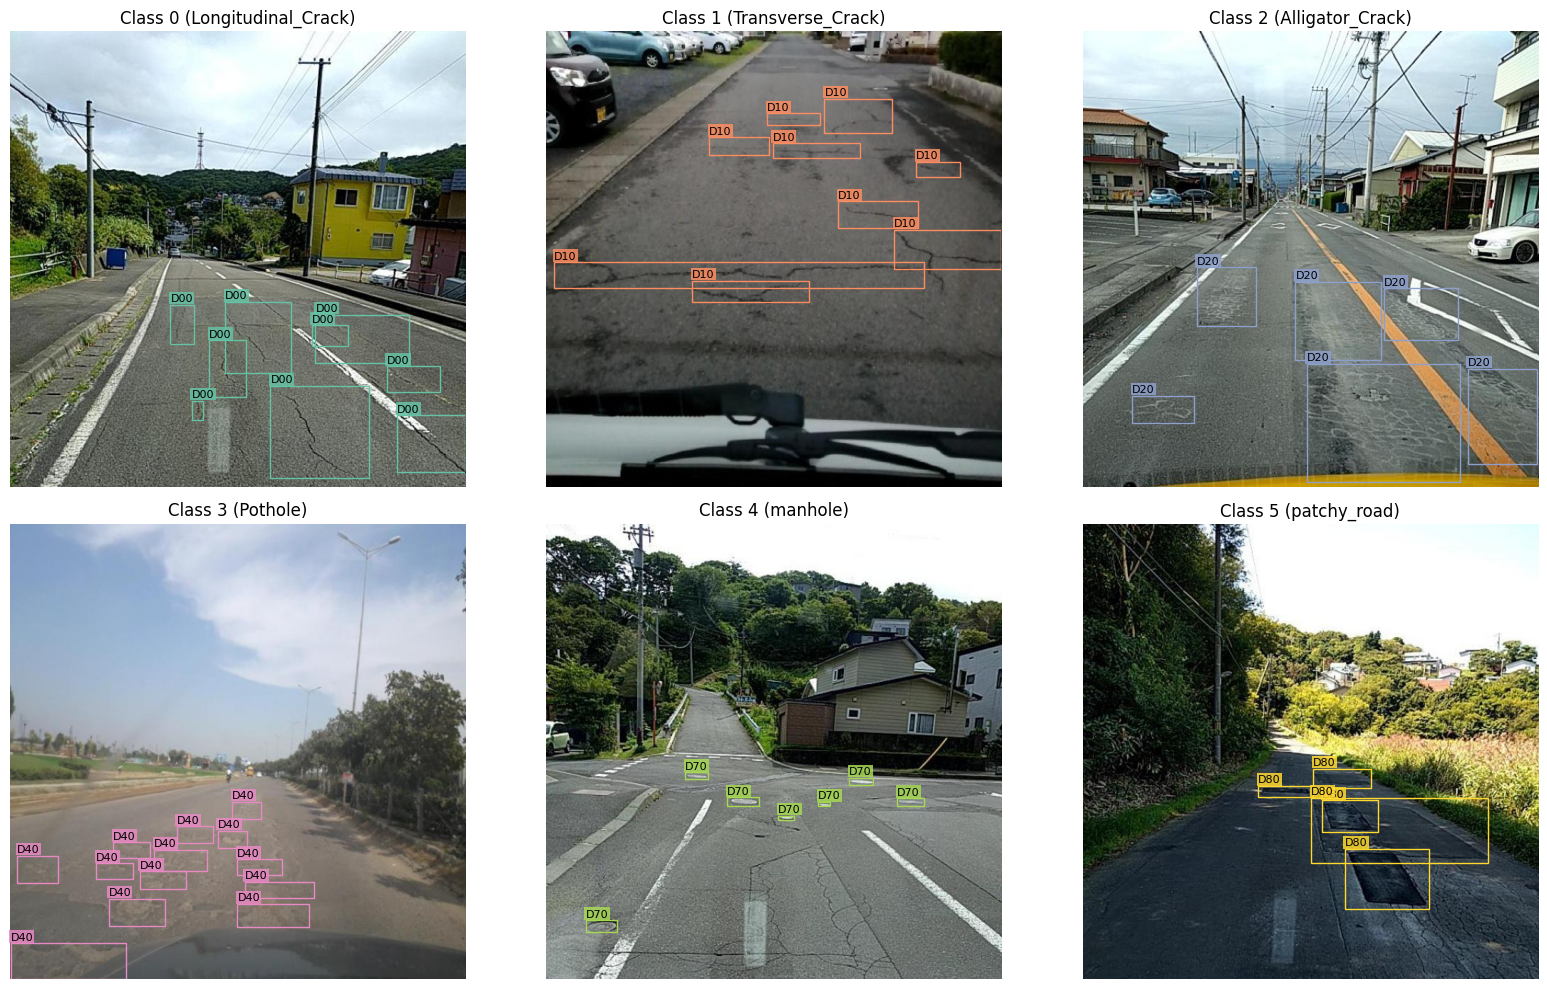
\includegraphics[width=\linewidth]{object_sample.png}
\caption{Contoh anotasi enam kelas pada data sumber, digunakan kembali dari proposal.}
\label{fig:contoh-kelas}
\end{figure}
Gambar~\ref{fig:contoh-kelas} memperlihatkan keragaman bentuk, ukuran, dan lokasi kotak pembatas. Visualisasi ini membantu menjelaskan objek yang menjadi masukan pelatihan. Panel yang dipilih tidak dimaksudkan untuk menyatakan distribusi kesulitan seluruh citra.

\subsection{Pembagian data dan distribusi anotasi}
Pembagian data sumber mengikuti rancangan sekitar 70:20:10 dengan stratifikasi multilabel untuk menjaga kemiripan proporsi kelas. Jumlah aktual citra pada setiap bagian disajikan pada Tabel~\ref{tab:pembagian}. Angka aktual digunakan sebagai dasar deskripsi eksperimen, bukan hasil pembulatan rasio rencana.
\begin{table}[H]
\centering
\caption{Inventaris pembagian citra dan anotasi sumber.}
\label{tab:pembagian}
\begingroup\fontsize{10}{13}\selectfont
\begin{tabularx}{\linewidth}{|X|r|r|r|}\hline
\rowcolor{black}\HeaderTabel{Bagian}&\HeaderTabel{Citra}&\HeaderTabel{Anotasi 6 kelas}&\HeaderTabel{Anotasi 4 kelas}\\\hline
Latih & 6.777 & 17.092 & 14.351\\\hline
Validasi & 1.898 & 4.773 & 3.996\\\hline
Uji & 995 & 2.425 & 2.035\\\hline
Total & 9.670 & 24.290 & 20.382\\\hline
\end{tabularx}\endgroup
\end{table}
Tabel~\ref{tab:pembagian} membedakan jumlah citra dari jumlah anotasi sebelum pemuatan validator. Log validasi mencatat penghapusan satu anotasi penutup saluran yang duplikat, sehingga evaluasi menggunakan 4.772 objek validasi. Perbedaan tersebut tidak mengubah inventaris 4.773 baris label atau jumlah 2.425 objek uji.

Distribusi kelas pada tiap bagian disajikan pada Tabel~\ref{tab:distribusi-kelas}.
\begin{table}[H]
\centering
\caption{Jumlah anotasi per kelas pada inventaris sumber.}
\label{tab:distribusi-kelas}
\begingroup\fontsize{10}{13}\selectfont
\begin{tabularx}{\linewidth}{|X|r|r|r|}\hline
\rowcolor{black}\HeaderTabel{Kelas}&\HeaderTabel{Latih}&\HeaderTabel{Validasi}&\HeaderTabel{Uji}\\\hline
Retak memanjang &4.555&1.257&635\\\hline
Retak melintang &3.219&897&446\\\hline
Retak buaya &4.385&1.245&642\\\hline
Lubang jalan &2.192&597&312\\\hline
Penutup saluran &2.270&645&321\\\hline
Jalan bertambal &471&132&69\\\hline
\end{tabularx}\endgroup
\end{table}
Tabel~\ref{tab:distribusi-kelas} memperlihatkan ketimpangan yang menjadi dasar pembobotan kelas. Pada data latih, rasio jumlah retak memanjang terhadap jalan bertambal sekitar 9,67. Bobot dihitung dari kolom latih saja menggunakan Persamaan~\eqref{eq:class-weight}, sehingga distribusi validasi, uji, dan target tidak menentukan pembobotan.

\subsection{Akuisisi dan anotasi data target}
Data primer diperoleh melalui perekaman menggunakan ponsel Android yang diarahkan ke jalan pada resolusi 1080p. Pengambilan dilakukan pada kedua arah perjalanan, terutama di Jalan Raya Bojongsoang serta jalan sekitarnya di Kabupaten Bandung. Video disampel pada interval satu bingkai per detik. Citra terpilih dianotasi oleh satu anotator menggunakan Roboflow dan dipotong pada bagian tengah menjadi $640\times640$ piksel.

Ekspor yang digunakan tersimpan sebagai RDD-indo-v4 dan memuat 307 citra pada bagian bernama \texttt{valid}. Metadata lokal mencatat proyek \texttt{rdd-indo-crop} versi 4. Dalam eksperimen ini, bagian tersebut digunakan sebagai data uji target. Nama \texttt{valid} dari ekspor tidak berarti bahwa data Indonesia digunakan untuk memilih bobot model.

Inventaris target berisi 502 anotasi, dengan 39 citra tanpa anotasi objek. Empat kelas kerusakan mencakup 481 anotasi, sedangkan jalan bertambal mencakup 21 anotasi. Tidak terdapat anotasi penutup saluran. Pemetaan kategori target ke identitas kelas sumber ditunjukkan pada Tabel~\ref{tab:pemetaan-target}.
\begin{table}[H]
\centering
\caption{Pemetaan kelas target dan jumlah anotasinya.}
\label{tab:pemetaan-target}
\begingroup\fontsize{10}{13}\selectfont
\begin{tabularx}{\linewidth}{|c|X|c|r|}\hline
\rowcolor{black}\HeaderTabel{ID target}&\HeaderTabel{Kategori}&\HeaderTabel{ID sumber}&\HeaderTabel{Anotasi}\\\hline
0 & Retak buaya &2&48\\\hline
1 & Retak memanjang &0&231\\\hline
2 & Jalan bertambal &5&21\\\hline
3 & Lubang jalan &3&70\\\hline
4 & Retak melintang &1&132\\\hline
\end{tabularx}\endgroup
\end{table}
Tabel~\ref{tab:pemetaan-target} memastikan bahwa perbedaan urutan label tidak mengubah makna kelas saat evaluasi. Seluruh 307 citra dipertahankan, termasuk citra tanpa anotasi. Kelas tanpa anotasi tidak diberi AP nol sebagai pengganti hasil evaluasi yang tidak tersedia.

Tambalan yang aus atau berbatas tidak teratur tetap termasuk kategori jalan bertambal pada anotasi target. Keterbatasan anotasi oleh satu orang dan cakupan lokasi perlu dipertimbangkan dalam interpretasi. Data ini digunakan sebagai pengujian lokal, bukan sampel yang mewakili seluruh jalan Indonesia.

\subsection{Representasi data dan augmentasi}
Anotasi menggunakan format YOLO yang memuat identitas kelas dan koordinat kotak ternormalisasi. Ukuran masukan model ditetapkan 640 piksel. Normalisasi intensitas dan penyesuaian masukan mengikuti pemuat data Ultralytics. Augmentasi hanya diterapkan pada pelatihan untuk membentuk variasi masukan.

Augmentasi utama mencakup Mosaic, MixUp, pembalikan horizontal, translasi, dan perubahan skala. Mosaic menggabungkan beberapa citra dalam satu masukan, sedangkan MixUp mencampurkan pasangan citra. Nilai konfigurasi aktual dicantumkan pada bagian pelatihan. Data uji digunakan tanpa augmentasi pelatihan agar evaluasi mengacu pada citra yang ditetapkan.

\section{Implementasi Model dan Pelatihan}
\subsection{Model bawaan dan rekonstruksi}
YOLOv8n, YOLOv12n, dan YOLO26n dimuat dari model bawaan dengan bobot pralatih. YOLOv8-PD dan YOLO-RD dibangun melalui definisi arsitektur lokal berdasarkan publikasi rujukan~\cite{Zeng2024,Wang2025}. Bobot YOLOv8n yang kompatibel dimuat ke kedua model rekonstruksi. Proses ini merupakan transfer parsial, bukan inisialisasi identik untuk seluruh parameter.

Rekonstruksi YOLOv8-PD mempertahankan struktur dasar ekstraksi fitur YOLOv8 dan menambahkan BoT serta LSKA setelah SPPF. Bagian penggabungan fitur menggunakan C2fGhost dan LSKA. Kepala deteksi menggunakan LSCDHead. Susunan ini merupakan implementasi lokal dari elemen rancangan YOLOv8-PD.

Rekonstruksi YOLO-RD menggunakan modul SOM pada \textit{backbone}, ARM pada fitur beberapa tingkat, serta WTHead dengan konvolusi berbasis wavelet. Fusi tambahan direalisasikan melalui \textit{upsample}, konkatenasi, dan konvolusi $1\times1$. Realisasi tersebut berbeda dari penjumlahan berbobot pada formulasi MAF asli~\cite{Wang2025}. Perbedaan ini membatasi klaim kesetaraan dengan model publikasi.

Kedua rekonstruksi memakai pengali kedalaman 0,33 dan lebar 0,25 pada skala nano. Namun, modul tambahan tetap menghasilkan jumlah parameter yang berbeda. Perbandingan karena itu menilai implementasi lengkap, bukan pengaruh topologi dengan kapasitas yang sepenuhnya dikendalikan.

\subsection{Konfigurasi pelatihan}
Argumen pelatihan setiap eksperimen disimpan bersama bobot model. Konfigurasi bersama pada pelatihan utama disajikan pada Tabel~\ref{tab:konfigurasi-latih}.
\begin{table}[H]
\centering
\caption{Konfigurasi pelatihan utama enam kelas.}
\label{tab:konfigurasi-latih}
\begingroup\fontsize{10}{13}\selectfont
\begin{tabularx}{\linewidth}{|X|X|}\hline
\rowcolor{black}\HeaderTabel{Pengaturan}&\HeaderTabel{Nilai}\\\hline
Ukuran masukan; ukuran batch &640 piksel; 16\\\hline
Batas epoch; patience &300; 40\\\hline
Seed; deterministic &42; aktif\\\hline
Optimizer &Pemilihan otomatis (\texttt{auto})\\\hline
Weight decay &0,0005\\\hline
Penjadwalan laju belajar &\textit{Cosine learning rate} aktif\\\hline
Mosaic; penutupan Mosaic &1,0; 10 epoch terakhir yang dijadwalkan\\\hline
MixUp; pembalikan horizontal &0,05; 0,5\\\hline
Translasi; perubahan skala &0,10; 0,50\\\hline
Rotasi &0 derajat\\\hline
Pembobotan kelas &Jumlah efektif sampel; $\beta=0{,}999$\\\hline
\end{tabularx}\endgroup
\end{table}
Tabel~\ref{tab:konfigurasi-latih} menyatakan argumen yang diberikan pada pelatihan, bukan jaminan bahwa semua model berhenti pada epoch yang sama. Pemilihan optimizer otomatis juga dapat menentukan pengaturan efektif yang berbeda. Nilai nominal laju belajar tidak diperlakukan sebagai bukti bahwa seluruh model menggunakan optimizer dan laju awal identik.

AMP diaktifkan pada ketiga model bawaan dan dinonaktifkan pada kedua rekonstruksi untuk pelatihan utama enam kelas. Pada eksperimen empat kelas, argumen yang tersimpan mencatat AMP aktif untuk kelima model. Perbedaan ini dicatat sebagai bagian konfigurasi perbandingan, sehingga ablasi tidak dinyatakan mengendalikan semua aspek pelatihan secara identik.

Bobot kelas dihitung dari frekuensi objek latih dan dinormalisasi menjadi rata-rata satu. Implementasi memasang bobot pada inisialisasi fungsi kerugian model agar tetap digunakan ketika pelatih membangun ulang model. Komponen klasifikasi menggunakan bobot tersebut, sementara jalur fungsi kerugian mengikuti arsitektur, termasuk jalur \textit{end-to-end} pada YOLO26n.

\subsection{Pemilihan bobot dan keterlacakan}
Bobot terbaik disimpan berdasarkan nilai \textit{fitness} validasi Ultralytics. Mekanisme penghentian dini menggunakan kesabaran 40 epoch. Pengujian sumber dan target memuat bobot terbaik dari proses ini. Tidak dilakukan pemilihan ulang \textit{checkpoint} berdasarkan skor target.

Artefak yang disimpan meliputi argumen pelatihan, riwayat metrik, bobot terbaik, serta hasil evaluasi per kelas. Konfigurasi tersimpan digunakan untuk mendeskripsikan pelaksanaan aktual. Hal ini diperlukan karena konstanta pada sel notebook yang telah diedit tidak selalu menggambarkan eksperimen sebelumnya.

\section{Protokol Pengujian dan Analisis}
\subsection{Evaluasi deteksi pada domain sumber}
Evaluasi akhir menggunakan 995 citra uji sumber. Metrik utama adalah mAP@0,5, dilengkapi mAP@0,5:0,95, presisi, \textit{recall}, dan F1. Hasil enam kelas menggambarkan tugas pelatihan utama. Rata-rata empat kelas kerusakan dilaporkan terpisah ketika digunakan untuk perbandingan antarkonfigurasi atau antardomain.

Evaluasi AP memakai ukuran masukan 640 piksel, ambang kepercayaan minimum 0,001, dan ambang IoU NMS 0,6 pada jalur yang menggunakan NMS. Ambang NMS tersebut bukan ambang IoU untuk menentukan TP. Penghitungan AP tetap menggunakan ambang pencocokan sesuai metrik yang dinyatakan.

F1 per kelas dihitung dari presisi dan \textit{recall} keluaran evaluator. Keluaran tersebut menggunakan ambang kepercayaan yang memaksimalkan kurva rerata F1 yang dihaluskan pada bagian data yang dievaluasi. Rata-rata makro dihitung menggunakan Persamaan~\eqref{eq:f1}. Dengan demikian, F1 ini merupakan ringkasan pada titik operasi hasil evaluasi, bukan kinerja pada ambang penerapan tetap yang dipilih sebelumnya.

\subsection{Evaluasi efisiensi}
Jumlah parameter dan GFLOPs dihitung dari \textit{checkpoint} akhir dalam bentuk model \textit{fused} pada masukan 640 piksel. Bentuk ini menggabungkan operasi tertentu untuk inferensi. Angkanya perlu dibedakan dari hitungan model sebelum penggabungan atau estimasi versi perangkat lunak lain.

Estimasi FPS menggunakan waktu rata-rata per citra yang dilaporkan validator. Perhitungannya dinyatakan pada Persamaan~\eqref{eq:fps}.
\begin{equation}
\operatorname{FPS}_{\mathrm{estimasi}}=\frac{1000}{t_{\mathrm{pra}}+t_{\mathrm{inferensi}}+t_{\mathrm{pasca}}}.
\label{eq:fps}
\end{equation}
Pada Persamaan~\eqref{eq:fps}, seluruh waktu menggunakan satuan milidetik per citra. Estimasi mencakup tiga tahap pemrosesan validator dan tidak berasal dari pengujian aplikasi terpisah. Pengukuran ini tidak mencakup percobaan khusus variasi batch atau protokol \textit{warm-up} mandiri.

Analisis efisiensi membandingkan ketepatan deteksi dengan parameter, GFLOPs, dan estimasi FPS. Pemilihan kandidat dibahas sesuai prioritas metrik, tanpa membentuk skor gabungan dengan bobot yang tidak ditetapkan dalam eksperimen. Kecepatan pada GPU pengujian tidak diproyeksikan langsung ke perangkat \textit{edge}.

\subsection{Perbandingan pelatihan empat dan enam kelas}
Eksperimen tambahan menghapus anotasi D70 dan D80 dari data sumber, dengan mempertahankan citra serta pembagian latih, validasi, dan uji. Citra yang menjadi tanpa anotasi tetap disertakan. Kelima arsitektur dilatih pada empat kelas kerusakan, dengan pembobotan yang dihitung kembali dari distribusi latih empat kelas.

Kinerja model empat kelas dibandingkan dengan model enam kelas pada D00, D10, D20, dan D40 saja. Prosedur ini menghindari perbandingan rata-rata atas himpunan kategori berbeda. Hasil dibaca sebagai perubahan yang teramati pada konfigurasi pelatihan, dengan memperhatikan perbedaan AMP dan sifat satu \textit{seed} eksperimen.

Analisis diagnostik tambahan menghitung kotak prediksi lubang dengan kepercayaan sedikitnya 0,25 yang bertumpang tindih dengan anotasi pengecoh pada IoU sedikitnya 0,5. Satu kotak prediksi dihitung sekali meskipun bertumpang tindih dengan beberapa anotasi. Sebaliknya, beberapa kotak prediksi dapat bertumpang tindih dengan objek yang sama. Hitungan ini bukan tingkat FP berbasis pencocokan unik antarobjek.

\subsection{Pengujian zero-shot pada target Indonesia}
Pengujian target menggunakan bobot enam kelas tanpa \textit{fine-tuning}, dengan pemetaan pada Tabel~\ref{tab:pemetaan-target}. Seluruh citra dipertahankan. Ambang kepercayaan minimum dan ukuran masukan mengikuti evaluasi sumber.

Perbandingan utama menggunakan mAP empat kelas kerusakan pada kedua domain. Penutup saluran dan jalan bertambal tidak masuk rata-rata tersebut. Evaluasi lima kelas yang menyertakan jalan bertambal diperlakukan sebagai analisis tambahan yang terpisah.

Penurunan absolut dan relatif dihitung melalui Persamaan~\eqref{eq:gap-absolut} dan~\eqref{eq:gap-relatif}.
\begin{equation}
\Delta_{\mathrm{abs}}=100\left(\operatorname{mAP}^{S}_{4}-\operatorname{mAP}^{T}_{4}\right).
\label{eq:gap-absolut}
\end{equation}
Persamaan~\eqref{eq:gap-absolut} menyatakan selisih dalam poin persentase ketika mAP sumber ($S$) dan target ($T$) ditulis pada skala nol sampai satu. Subskrip empat menegaskan bahwa kedua rata-rata menggunakan kategori yang sama.
\begin{equation}
\Delta_{\mathrm{rel}}=100\left(1-\frac{\operatorname{mAP}^{T}_{4}}{\operatorname{mAP}^{S}_{4}}\right)\%.
\label{eq:gap-relatif}
\end{equation}
Persamaan~\eqref{eq:gap-relatif} menyatakan penurunan sebagai persentase terhadap kinerja sumber, selama penyebut lebih besar dari nol. Kedua ukuran merangkum kesenjangan kinerja antardataset. Nilainya bukan ukuran langsung jarak distribusi atau bukti pengaruh kausal pencahayaan, tekstur, dan lokasi.

\subsection{Batas interpretasi}
Perbandingan satu \textit{seed} belum mengukur variasi antarulangan, sehingga selisih metrik tidak dinyatakan signifikan. Rekonstruksi, transfer parsial, dan perbedaan konfigurasi membatasi klaim pengaruh modul secara kausal. Cakupan target lokal dan anotasi oleh satu orang juga membatasi generalisasi. Contoh visual serta hitungan tumpang tindih digunakan sebagai bukti deskriptif.
